\documentclass{beamer}
\mode<presentation>

\usepackage[english]{babel}
\usepackage[latin1]{inputenc}
\usepackage{times}
\usepackage[T1]{fontenc}
\usepackage{graphicx}
\usepackage[justification=centering]{caption}
\usepackage{subcaption}
\usepackage{url}
\usepackage{setspace}
\usepackage{color}
\usepackage{algorithm2e}

\usepackage{listings}
\lstset{breaklines=true}
%\lstset{upquote=true}
\lstset{basicstyle= \small}%\footnotesize}

\usepackage{tikz}
\usetikzlibrary{trees}

\usepackage{pgfpages}

\addtobeamertemplate{navigation symbols}{}{%
    \usebeamerfont{footline}%
    \usebeamercolor[fg]{footline}%
    \hspace{1em}%
    \insertframenumber%/\inserttotalframenumber
}

\AtBeginSection[]{
  \begin{frame}
  \vfill
  \centering
  \begin{beamercolorbox}[sep=8pt,center,shadow=true,rounded=true]{title}
    \usebeamerfont{title}\insertsectionhead\par%
  \end{beamercolorbox}
  \vfill
  \end{frame}
}

\usepackage{hyperref}

\newcommand{\orka}{\textit{Orka}}
\newcommand{\petra}{\textit{PETrA}}

\newcommand{\monkeyrunner}{\texttt{monkeyrunner}}
\newcommand{\apk}{\texttt{apk}}
\newcommand{\logcat}{\texttt{logcat}}
\newcommand{\netstats}{\texttt{netstats}}

\newcommand{\lv}{Linares-Vasquez et al.}
\setbeameroption{show notes on second screen=right}
\title[Project presentation]{\textsc{Hardware usage accounting and source-line level energy estimates on Android}}
\author{Alexandre \textsc{Cornet}\\ {\footnotesize supervised by Dr. Anandha \textsc{Gopalan}}}
\institute{Imperial College London}
\date{September 2017}
\pgfdeclareimage[height=0.5cm]{university-logo}{figures/imperial.pdf}
\logo{\pgfuseimage{university-logo}}
\begin{document}
\begin{frame}
\titlepage
\note[enumerate]{
\item building an energy profiler for Android Applications}
\end{frame}
%
\iffalse
\begin{frame}
\framtitle
\tableofcontents%[pausesections]
}
\end{frame}
\fi
%
%%%%%%%%%%%%%%% PROBLEM
%
\section{Problem}
% FIXME text box on top of frame
\begin{frame}{Energy efficiency matters}
\begin{columns}
\begin{column}{0.5\textwidth}
\begin{figure}
        
\includegraphics[width=\textwidth]{figures/angry_feedback_1.png}
\end{figure}
\end{column}
\begin{column}{0.5\textwidth}
\begin{figure}
        
\includegraphics[width=\textwidth]{figures/angry_feedback_2.png}
\end{figure}
\end{column}
\end{columns}
\end{frame}
%
%%%%%%%%%%%%%%% RELATED WORK
%
\section{Related work}
\begin{frame}{Energy-profilers}
\begin{itemize}
\item Highlight the energy-greediest parts of the code
\item Three types:
\begin{enumerate}
\item hardware-based
\item model-based
\item software-based
\end{enumerate}
\item Yet, \alert{no solution accessible} to the majority of developers
\end{itemize}
\end{frame}
%
%
\begin{frame}{What's missing?}
A software-based energy-profiler:
\begin{enumerate}
\item providing hardware-usage and \alert{tail-energy} accounting,
\item providing \alert{source-line level} estimates,
\item open-sourced.
\end{enumerate}
\end{frame}
%
%%%%%%%%%%%%%%% ORKA
%
\section{Orka}
\begin{frame}{\orka{}: overview}
\begin{itemize}
\item Input: Tested \apk{} file and \monkeyrunner{} test script
\item Output: Energy estimates at the method-level
\item Main assumption:
$$ cost(routine) = \sum_{API \in routine} cost(API)$$
\item Rely on \alert{instrumentation} and on the Android emulator
\end{itemize}
\end{frame}
%
%
\begin{frame}{\orka{}: workflow}
\begin{figure}
        \includegraphics[width=\textwidth]{figures/orkaworkflow.pdf}
\end{figure}
\end{frame}
%
%
\begin{frame}
  \vfill
  \centering
  \begin{beamercolorbox}[sep=8pt,center,shadow=true,rounded=true]{title}
    \usebeamerfont{title}Demo\par%
  \end{beamercolorbox}
  \vfill
\end{frame}
%%%%%%%%%%%%%%% HARDWARE
%
\section{Hardware-usage and tail-energy accounting}
\begin{frame}{Tail-energy}
\begin{columns}
\begin{column}{0.5\textwidth}
\begin{figure}
% FIXME better breakdown
	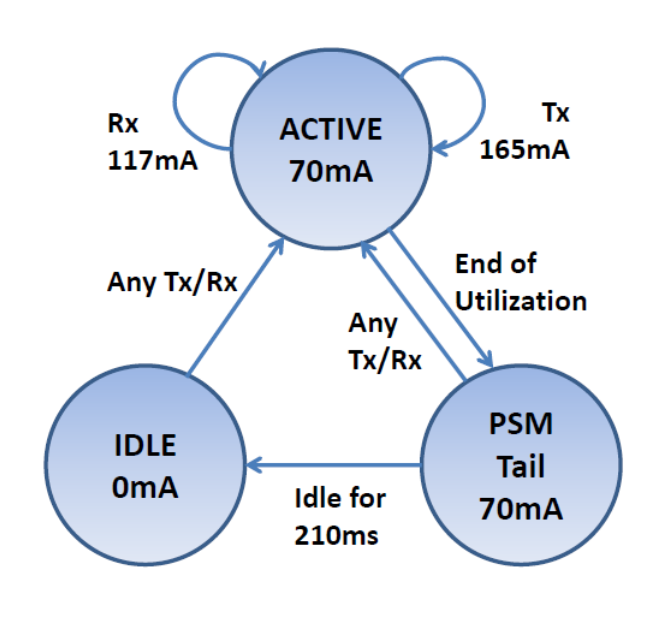
\includegraphics[width=\textwidth]{figures/wifi_statemachine.png} 
\end{figure}
\end{column}
\pause
\begin{column}{0.5\textwidth}
\begin{itemize}
\item Tail-energy: the component stays in a high power-state \alert{after} completing a task.
\end{itemize}
\end{column}
\end{columns}
\end{frame}
%
%
\begin{frame}{Problem}
\begin{columns}
\begin{column}{0.5\textwidth}
\begin{figure}
% FIXME better breakdown
	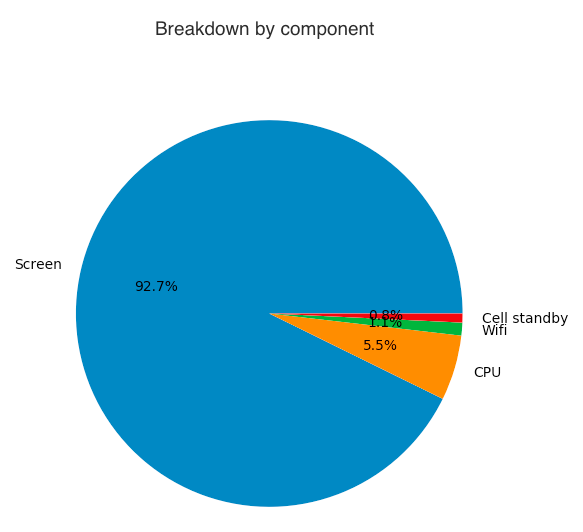
\includegraphics[width=\textwidth]{figures/hw_breakdown.png} 
\end{figure}
\end{column}
\begin{column}{0.5\textwidth}
The breakdown by component:
\begin{itemize}
\item is \alert{difficult to interpret},
\item doesn't account for \alert{tail-energy}.
\end{itemize}
\end{column}
\end{columns}
\end{frame}
%
%
\begin{frame}{Aims (1/2)}
\begin{itemize}
\item Map hardware-usage back to the code
\item Account for tail-energy
\end{itemize}
\vskip0pt plus.5fill
\begin{block}{Simplifications}
\begin{itemize}
\item Only for Wi-Fi
\item At the method level
\item Focus on time ($E= P \Delta_t$)
\end{itemize}
\end{block}
\end{frame}
%
%
\begin{frame}[fragile]{Aims (2/2)}
\begin{block}{Desired output}
%[frame=single, emph={cout}, emphstyle={\color{blue}}]
\begin{lstlisting}
MainActivity.<init> {ACTIVE: 0.0, IDLE: 0.01,
  TAIL: 0.0}
MainActivity$SendGet.run {ACTIVE: 1.57, IDLE: 0.84,
  TAIL: 1.62}
\end{lstlisting}
\end{block}         
\end{frame}
%
%
\begin{frame}{Technical challenges}
\begin{block}{Goal}
\begin{itemize}
\item \alert{Correlate} the Wi-Fi energy activity with routine calls
\end{itemize}
\end{block}
\begin{block}{Requirements}
\begin{itemize}
\item Log when routines start and terminate
\item Log when Wi-Fi switches from one state to another
\end{itemize}
\end{block}
\end{frame}
%
%
\begin{frame}[fragile]{Monitoring the call-stack}
\begin{columns}
\begin{column}{0.6\textwidth}
% 09-04 12:52:26.642 1474 9092 I orka: Ind
\begin{lstlisting}
12:52:26.642 entering foo
12:52:26.742 	API call api1
12:52:26.842 entering bar
12:52:26.942 	API call api2
12:52:27.042 exiting bar
12:52:27.142 exiting foo
\end{lstlisting}
\end{column}
\begin{column}{0.4\textwidth}
\begin{itemize}
\item Extended the injector to \alert{log when methods return}
\item Used \logcat{} in \texttt{threadtime} mode to \alert{include timestamps}
\end{itemize}
\end{column}
\end{columns}
\end{frame}
%
%
\begin{frame}[fragile]{Monitoring the energy state of Wi-Fi}
% FIXME two col, add state machine
\begin{itemize}
\item We need to monitor what trigger transitions: \alert{network traffic}.
\item Leverage \texttt{proc/net/xt\_qtaguid/stats}
\end{itemize}
\vskip0pt plus.5fill
%[frame=single]
\begin{lstlisting}
idx iface uid_tag_int cnt_set rx_bytes rx_packets tx_bytes tx_packets
2 wlan0 0 0 200888 1096 79636 888
3 wlan0 0 1 0 0 0 0
\end{lstlisting}
\end{frame}
%
%
\begin{frame}{Network monitoring: algorithm}
\begin{small}
\begin{algorithm}[H]
%\KwIn{Active ADB connection to an actual device}
\KwOut{Logs of the energy states of the Wi-Fi antenna}
Get first network statistics $S_0$ at current time $t_0$\;
$state \leftarrow \texttt{IDLE}$\;
\While{True}{
Get network statistics $S_1$ at current time $t_1$\;
\uIf{$S_0 \neq S_1$}
{$state \leftarrow \texttt{ACTIVE}$\;}
\ElseIf{state = \texttt{ACTIVE}}{$state \leftarrow \texttt{TAIL}$\;$tail_{start} \leftarrow t_0$\;}
\If{$state = \texttt{TAIL}$ {\normalfont \textbf{and}} $t_1 - tail_{start} \geq tail_{time}$}
{Log $(t_0, state)$\;
$t_0 \leftarrow tail_{start} + tail_{time}$\;
$state \leftarrow \texttt{IDLE}$\;}
Log $(t_0, state)$\;
$t_0 \leftarrow t_1$, $S_0 \leftarrow S_1$\;
}
\end{algorithm}
\end{small}
\end{frame}
%
%
\begin{frame}
  \vfill
  \centering
  \begin{beamercolorbox}[sep=8pt,center,shadow=true,rounded=true]{title}
    \usebeamerfont{title}Demo\par%
  \end{beamercolorbox}
  \vfill
\end{frame}
%
%
\begin{frame}[fragile]{Network monitoring: results}
\begin{lstlisting}
1503657227.287407 ACTIVE
1503657227.323574 TAIL
1503657227.359771 TAIL
1503657227.394717 TAIL
1503657227.428777 ACTIVE
1503657227.467203 TAIL
1503657227.518874 ACTIVE
1503657227.589833 ACTIVE
1503657227.644556 TAIL
1503657227.681700 TAIL
1503657227.716493 TAIL
1503657227.753575 TAIL
1503657227.789498 TAIL
1503657227.829724 TAIL
1503657227.864556 IDLE
1503657227.882524 IDLE
\end{lstlisting}
\end{frame}
%
%
\begin{frame}[fragile]{Network analyser: principle}
\begin{columns}
\begin{column}{0.5\textwidth}
% 09-04 12:52:26.642 1474 9092 I orka: Ind
\begin{lstlisting}
12:52:26.642 entering foo
12:52:26.742 	...
12:52:26.842 entering bar
12:52:26.942 	...
12:52:27.042 exiting bar
12:52:27.142 exiting foo
\end{lstlisting}
\end{column}
\begin{column}{0.5\textwidth}
\begin{lstlisting}
1503657227.589833 ACTIVE
1503657227.644556 TAIL
1503657227.681700 TAIL
1503657227.716493 TAIL
1503657227.753575 TAIL
1503657227.864556 IDLE
\end{lstlisting}
\end{column}
\end{columns}
\vskip0pt plus.5fill
\begin{itemize}
\item Replay both logs
\item Tally time spent in each mode for all methods
\end{itemize}
\end{frame}
%
%
\begin{frame}[fragile]{Network analyser: results}
\begin{lstlisting}
MainActivity.<init> {ACTIVE: 0.0, IDLE: 0.01,
  TAIL: 0.0}
MainActivity$SendGet.run {ACTIVE: 1.57, IDLE: 0.84,
  TAIL: 1.62}
\end{lstlisting}
\end{frame}
%
%%%%%%%%%%%%%%% CONCLUSION
%
\section{Conclusion}
\begin{frame}{Summary}
This work stands as the first software-based tool:
\begin{enumerate}
\item accounting for \alert{tail-energy},
\item providing \alert{source-line level} energy estimates,
\item available as an \alert{open-source} application.
\end{enumerate}
\vskip0pt plus.5fill
{\small \orka{} is available at \url{https://github.com/acornet/orka}}
\end{frame}
%
%
\begin{frame}{Outlook}
\begin{itemize}
\item Source line-level energy estimates
\item Evaluation of \orka{}'s accuracy using \petra{}
\item Preparatory work: refactoring process and usability features
\end{itemize}
\end{frame}
%
%
\begin{frame}
  \vfill
  \centering
  \begin{beamercolorbox}[sep=8pt,center,shadow=true,rounded=true]{title}
    \usebeamerfont{title}Thank you\par%
  \end{beamercolorbox}
  \vfill
\end{frame}
\end{document}
